\section{Integrations}
Spring XD integration modules are Message Endpoints \cite{enterprise-integration-pattern-message-endpoint} 
that are responsible for sending data to and receiving data from external applications.
There are three types of message endpoints: sources, sinks and batch jobs.
A source is the entry point for data into the stream. A sink is the module that dispatches
the stream's results to an external application or storage system. Batch jobs are used to
execute batch processing steps on a set of data.

\par

Spring XD offers a suite of 23 sources, 24 sinks and 9 jobs that are ready to use at startup.
These modules integrate with a variety of well known and popular data stores
and processing systems such as JDBC, HDFS, MongoDB, Spark, and Sqoop.
If an existing module does not meet the needs of a given use case, Spring XD supports custom
modules.

\par

\subsection{Module Integrations: Source}
Source modules receive inbound data and convert it to messages for
use by modules in a stream or by a batch job.
There are two source types: poller and event driven.  A poller source is based on the polling
consumer pattern \cite{enterprise-integration-pattern-pollingconsumer}. It
will poll an external application (such as a web service, FTP server, database) for data at a
configurable interval. An event driven source is based on the event driven
consumer pattern \cite{enterprise-integration-pattern-eventdrivenconsumer} which will
open a port to listen for incoming data that is pushed from an external application.

\par

Spring XD uses Spring Integration \cite{spring-integration-reference} as its foundation
for implementing source and sink modules. Integration modules are
comprised minimally of one channel and an integration bean.  In the case of a source module
there is an "output" channel to dispatch messages transmitted by the integration bean to
the stream (see figure~\ref{fig:sourcembc}.)

\par

\begin{figure}[ht]
\centering
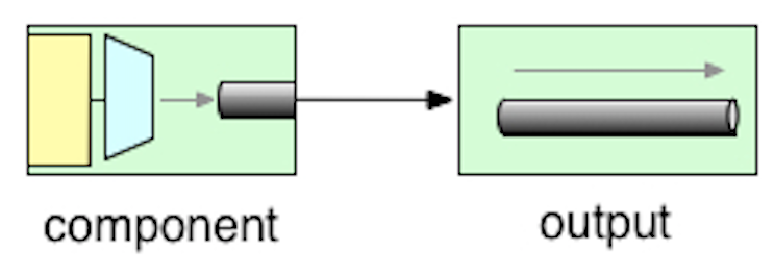
\epsfig{file=integration-module-output-channel.eps, height=.8in, width=2in}
\caption{Source Module Basic Components}
\label{fig:sourcembc}
\end{figure}

\subsection{Module Integrations: Sink}
Sink modules convert and deliver messages from a stream in a format consumable by an external application.
There are two types of sinks: counter/gauge and delegate.
A counter/gauge is a specialized sink that increments a field on a datastore every time a
message is received. (Refer to the Analytics section for more information.)  A delegate
sink translates messages to the format expected by the external application.
After transforming the message, the resulting data is sent to the external application.

\par

The basic sink is comprised of a "input" channel and an integration bean.
The input channel receives all messages from the stream and dispatches
messages to the integration bean (see figure~\ref{fig:sinkmbc}.) It is the responsibility of
the integration bean to implement retry behavior in cases of failure. The sinks included
in Spring XD have configurable options for retries.

\par

\begin{figure}
\centering
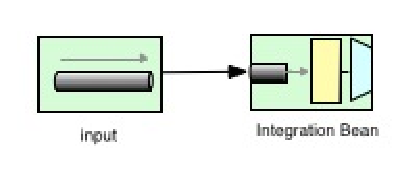
\epsfig{file=integration-module-input-channel.eps, height=.8in, width=2in}
\caption{Sink Module Basic Components}
\label{fig:sinkmbc}
\end{figure}

\subsection{Module Integrations: Job}
Spring XD uses Spring Batch \cite{spring-batch-reference} as the foundation for implementing
job modules.  Jobs enables users to execute enterprise batch processes within Spring XD.
Jobs are typically used when running long lasting tasks that have transactional requirements.
Thus in cases that the job fails, a job can be designed to be restarted and
pickup where it left off or rollback the changes that were in transaction.

\par

A job is typically comprised of a job definition along with the supporting
bean(s) as shown in figure~\ref{fig:batchmbc}.
In some cases the job definition alone is sufficient to implement the desired behavior.

\par

\begin{figure}
\centering
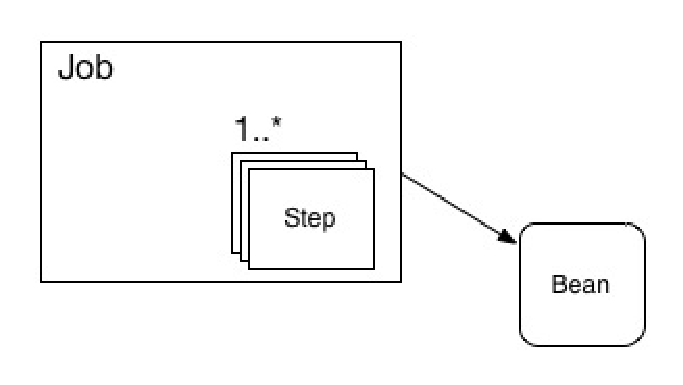
\epsfig{file=integration-batch.eps, height=.8in, width=2in}
\caption{Batch Basic Components}
\label{fig:batchmbc}
\end{figure}

\subsection{Deployment}
Integration modules are deployed in the modules directory and are segregated in
subdirectories by type: modules/source, modules/sink and modules/job.
These modules are dynamically loaded when a stream or job is deployed that requires that
specific module.

\par

\subsection{Integration Examples}
With the advent of microservices \cite{microservices-pattern} applications are becoming 
evermore integrated.  In cases where an application needs access to microservices but does not 
have the capability to transmit the request via the API presented, or an application needs to 
take the results of a microservice and transmit it to  an external application in the application's 
accepted format, XD can bridge that chasm. 
An example of this would be if we needed a service that would receive sensor data via mqtt 
and write that the data to hdfs. The following stream would be used to do this: "mqtt|hdfs".
Another example of this would be a scenario if a database is being updated by a service 
but while the database is updated we need to update a mongo collection 
with this data.  This can be done by creating a stream that would monitor a table(s) 
retrieve changes and write the results to the mongo collection.  This would be 
represented by the following stream: 
"jdbc --fixedDelay=1 --split=1 --query='select * from testfoo where tag = 0' --update=
'update testfoo set tag=1 where fooid in (:fooid)'|log" 
\begin{description}
\item[Example Source] \hfill \\
jdbc - is a poller source that will execute a query against a database and generate a 
message for each row that is retrieved.  \cite{jdbc-module}
mqtt - is a event driven source that awaits for mqtt messages to be received once the message is
 received the payload of the message is sent as an XD message to the next module in the 
 stream.  \cite{mqtt-module}
\item[Example Sink] \hfill \\
Mongo - The Mongo sink writes messages into a Mongo collection \cite{mongo-module}
hdfs - writes messages to the specified location on a hadoop instance. \cite{hadoop-hdfs-module}
\item[Example Job] \hfill \\
filejdbc -A module which loads CSV files into a JDBC table\par
\end{description}
